% !TEX root = Apostila GP.tex

\capitulo{Qualidade}

\secao{Objetivos e características}

O gerenciamento da qualidade do projeto inclui processos e atividades da organização executora que determinam políticas, objetivos e responsabilidades referentes a qualidade, a fim de que o projeto satisfaça as necessidades para o qual foi empreendido. O gerenciamento da qualidade do projeto utiliza políticas e procedimentos para implementar, dentro do contexto do projeto, o sistema de gestão da qualidade da organização e suporta atividades de melhoria contínua de processos. O gerenciamento da qualidade do projeto trabalha para garantir que os requisitos do projeto, incluindo os requisitos do produto, sejam alcançados e validados.

Os processos que fazem parte do gerenciamento da qualidade, representados na Figura \ref{fig:proc:ger:qualidade}, podem ser resumidos em:

\begin{description}
	
	\item[\textbf{Planejar o Gerenciamento da Qualidade}]: identificar os requisitos e/ou padrões para o projeto e suas entregas e documentar como o projeto irá atendê-los.
	
	\item[\textbf{Realizar a garantia da qualidade}]: auditar os requisitos de qualidade e os resultados das medidas do controle de qualidade para garantir que os padrões apropriados de qualidade e as definições operacionais estejam sendo utilizadas.
	
	\item[\textbf{Controlar a qualidade}]: monitorar e registrar os resultados de execução das atividades de qualidade para avaliar o desempenho e recomendar as mudanças necessárias.

\end{description}

\begin{figure}[!h]
	\centering
	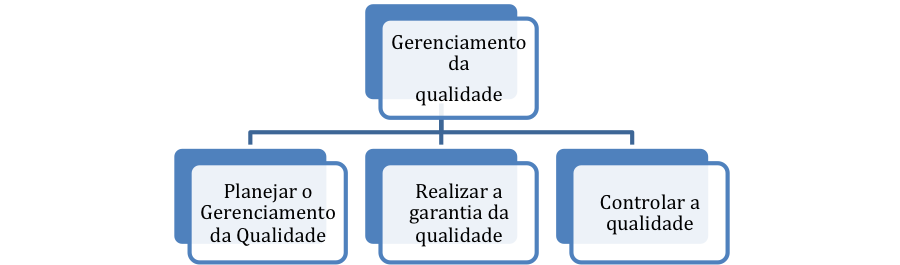
\includegraphics[scale=0.75]{Figuras/gerenciamento_qualidade.png}
	\caption{Processos do gerenciamento da qualidade}
	\label{fig:proc:ger:qualidade}
\end{figure}

\secao{Planejar o Gerenciamento da Qualidade}

O plano de gerenciamento da qualidade é o processo de identificar os requisitos e/ou padrões para o projeto e suas entregas e documentar como o projeto irá atendê-los.

O processo de planejar o gerenciamento da qualidade está representado na Figura \ref{fig:qualidade:plan:efts} e será descrito a seguir.

\begin{figure}[!h]
	\centering
	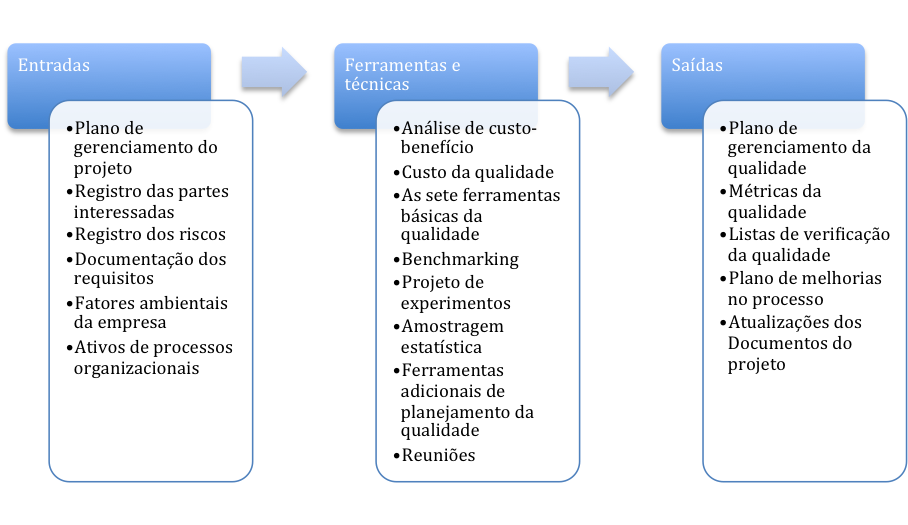
\includegraphics[scale=0.5]{Figuras/qualidade_efts_planejar.png}
	\caption{Planejar o gerenciamento da qualidade: entradas, ferramentas, técnicas e saídas}
	\label{fig:qualidade:plan:efts}
\end{figure}

\section{Entradas}

\begin{description}
	
	\item[Plano de gerenciamento do projeto:] inclui informações utilizadas no desenvolvimento do plano de gerenciamento da qualidade (linha de base do escopo, do cronograma e do custo, entre outros documentos).
	
	\item[Registro das partes interessadas:] auxilia na identificação de quem possua um interesse particular ou tenha um impacto na qualidade.
	
	\item[Registro dos riscos:] contém informações sobre ameaças e oportunidades que possam impactar nos requisitos de qualidade.
	
	\item[Documentação dos requisitos:] capturam os requisitos que o projeto deve atender pertinentes às expectativas das partes interessadas.
	
	\item[Fatores ambientais da empresa:] regulamentações de agências governamentais, regras, padrões e diretrizes específicas para uma área de aplicação, condições de operação ou de trabalho do projeto ou das entregas que possam afetar a qualidade do projeto, percepções culturais que possam influenciar as expectativas sobre a qualidade, etc.
	
	\item[Ativos de processos organizacionais:] políticas, procedimentos e diretrizes organizacionais, bancos de dados históricos, lições aprendidas, etc.
	
\end{description}

\section{Ferramentas e técnicas}

\begin{description}

	\item[Análise de custo-benefício:] compara o custo de cada atividade da qualidade com seu benefício esperado.
	
	\item[Custo da qualidade:] são os custos usados para prevenir a não conformidade, ou seja, o dinheiro gasto durante o projeto para evitar falhas. Entre eles:
	
	\begin{itemize}
		
		\item Custos de conformidade
					
		\begin{itemize}

			\item Prevenção de custos (Fabricar um produto de qualidade)
			
			\begin{itemize}
				
				\item Treinamento;
				
				\item Documentar processos;
				
				\item Equipamento;
				
				\item Tempo para executar do modo correto.
				
			\end{itemize}
			
			\item Custos de avaliação (Avaliar a qualidade)
			
			\begin{itemize}
				
				\item Testes;
				
				\item Perda de teste destrutivo;
				
				\item Inspeções.
				
			\end{itemize}
			
		\end{itemize}
	
		\item Custos de não conformidade
		
		\begin{itemize}
		
			\item Custos de falhas internas (Falhas encontradas pelo projeto)
			
			\begin{itemize}
				
				\item Retrabalho;
				
				\item Descarte.
				
			\end{itemize}
			
			\item Custos de falhas externas (Falhas encontradas pelo cliente)	
			
			\begin{itemize}
				
				\item Responsabilidades;
				
				\item Trabalho de garantia;
				
				\item Perda de negócios.

			\end{itemize}
						
		\end{itemize}
	
	\end{itemize}

	\item[As sete ferramentas básicas da qualidade:] também conhecidas como \textit{7QC Tools}.
	
		\begin{itemize}
			\item Diagrama de causa-efeito
			\item Fluxograma
			\item Folha de verificação
			\item Histograma
			\item Diagrama de Pareto
			\item Gráfico de controle
			\item Diagrama de dispersão			
		\end{itemize}
	
	\item[Benchmarking:] é o processo de comparar os métodos de trabalho em relação às melhores práticas e resultados com o propósito de identificar mudanças que levem a resultados de melhor qualidade.
	
	\item[Projeto de experimentos:] método estatístico que ajuda a identificar quais fatores podem influenciar variáveis específicas de um produto ou processo em desenvolvimento.
	
	\item[Amostragem estatística:] tem como objetivo fazer generalizações sobre uma população com base nos dados de uma amostra.
	
	\item[Ferramentas adicionais de planejamento da qualidade:] alguns exemplos:
	
	\begin{itemize}
		
			\item Brainstorming;
			
			\item Técnica de grupo nominal;
			
			\item Diagramas Matriciais;
			
			\item Matriz de priorização.
			
	\end{itemize}
		
	\item[Reuniões:] utilizadas para auxiliar no desenvolvimento do plano de gerenciamento da qualidade.
		
\end{description}

\section{Saídas}

\begin{description}
	
	\item[Plano de gerenciamento da qualidade:] descreve como as políticas de qualidade da organização serão implementadas.
	
	\item[Plano de melhoria de processos:] detalha os passos para analisar os processos de gerenciamento de projeto e desenvolvimento de produto para identificar atividades que possam aumentar seus valores.
	
	\item[Métricas da qualidade:] descreve um atributo do projeto ou do produto e como o processo de controle de qualidade irá mensurá-lo.
	
	\item[Listas de verificação da qualidade:] utilizada para verificar se um conjunto de passos requeridos foram executados.
	
	\item[Atualizações dos Documentos do projeto:] registro de partes interessadas, matriz de atribuição de responsabilidades, EAP e dicionário da EAP, etc.
		
\end{description}

\secao{Realizar a garantia da qualidade}

Processo de auditar os requisitos de qualidade e os resultados das medidas do controle de qualidade para garantir que os padrões apropriados de qualidade e as definições operacionais estejam sendo utilizadas.

O processo de realizar a garantia da qualidade está representado na Figura \ref{fig:qualidade:gar:efts} e será descrito a seguir.

\begin{figure}[!h]
	\centering
	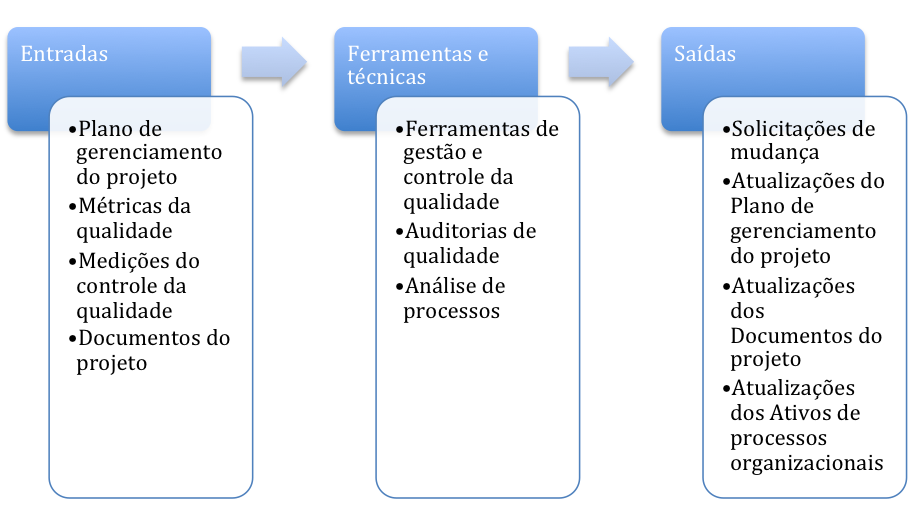
\includegraphics[scale=0.5]{Figuras/qualidade_efts_realizar.png}
	\caption{Realizar a garantia da qualidade: entradas, ferramentas, técnicas e saídas}
	\label{fig:qualidade:gar:efts}
\end{figure}

\section{Entradas}

\begin{description}

	\item[Plano de gerenciamento da qualidade:] descreve a abordagem da garantia da qualidade e da melhoria contínua de processos do projeto.
	
	\item[Plano de melhoria dos processos:] as atividades de garantia da qualidade do projeto devem ser consistentes e apoiar os planos de melhoria de processos da organização.
	
	\item[Métricas da qualidade:] indicam os atributos que devem ser mensurados e as variações toleráveis.
	
	\item[Medições do controle da qualidade:] resultados das atividades de controle da qualidade.
	
	\item[Documentos do projeto:] documentos que possam influenciar no trabalho da garantia da qualidade.
		
\end{description}

\section{Ferramentas e técnicas}

\begin{description}
	
	\item[Ferramentas de gestão e controle da qualidade:] alguns exemplos:
	
	\begin{itemize}
		
		\item Diagrama de afinidades;
		
		\item Gráfico de programa de decisão de processo (PDPC);
		
		\item Gráfico de inter relacionamento;
		
		\item Diagramas de árvore;
		
		\item Matrizes de priorização;
		
		\item Diagramas de rede;
		
		\item Diagramas de matriz.
		
	\end{itemize}
	
	\item[Auditorias de qualidade:] processo estruturado e independente que determina se as atividades do projeto estão em conformidade com as políticas, processos e procedimentos da organização e do projeto.
	
	\item[Análise de processos:] segue os passos delineados no plano de melhoria de processos para identificar o que precisa ser melhorado.
		
\end{description}

\section{Saídas}

\begin{description}
	\item[Solicitações de mudança:] podem ser geradas para avaliação das melhorias recomendadas.
	
	\item[Atualizações do Plano de gerenciamento do projeto:] planos de gerenciamento da qualidade, escopo, tempo e custo, entre outros.
	
	\item[Atualizações dos Documentos do projeto:] relatórios de auditoria da qualidade, planos de treinamento, etc.
	
	\item[Atualizações dos Ativos de processos organizacionais:] padrões de qualidade, sistemas de gerenciamento da qualidade, etc.
	
\end{description}

\secao{Controlar a qualidade}

Processo de monitorar e registrar os resultados de execução das atividades de qualidade para avaliar o desempenho e recomendar as mudanças necessárias.

O processo de controlar a qualidade está representado na Figura \ref{fig:qualidade:controlar:efts} e será descrito a seguir.

\begin{figure}[!h]
	\centering
	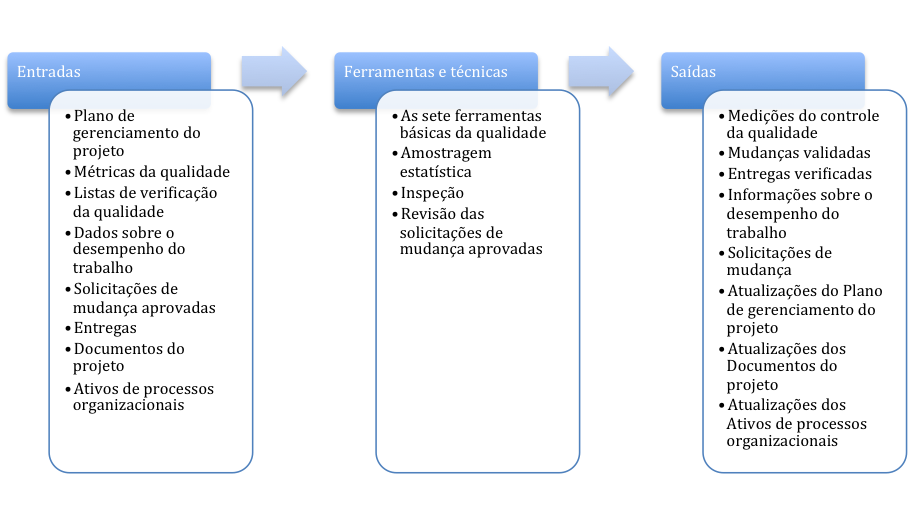
\includegraphics[scale=0.5]{Figuras/qualidade_efts_controlar.png}
	\caption{Controlar a qualidade: entradas, ferramentas, técnicas e saídas}
	\label{fig:qualidade:controlar:efts}
\end{figure}

\section{Entradas}

\begin{description}

	\item[Plano de gerenciamento do projeto:] utiliza o plano de gerenciamento da qualidade que descreve como será feito o controle da qualidade.
	
	\item[Métricas da qualidade:] descrição dos atributos e formas de mensurá-los.
	
	\item[Listas de verificação da qualidade:] lista estruturada que auxilia na verificação do trabalho do projeto e suas entregas.
	
	\item[Dados sobre o desempenho do trabalho:] permite confrontar o que foi planejado com os dados reais de trabalho.
	
	\item[Solicitações de mudança aprovadas:] podem incluir reparo de defeitos, métodos de trabalho revisados e cronograma revisado.
	
	\item[Entregas:] produto, resultado ou capacidade única e verificável do projeto que resulta em uma entrega validada requerida pelo projeto.
	
	\item[Documentos do projeto:] acordos, relatórios de auditoria da qualidade, planos de treinamento, etc.
	
	\item[Ativos de processos organizacionais:] políticas e padrões de qualidade da organização, diretrizes padrões de trabalho, etc.
	
\end{description}

\section{Ferramentas e técnicas}

\begin{description}
	
	\item[As sete ferramentas básicas da qualidade:] também conhecidas como \textit{7QC Tools}.
	
	\begin{itemize}
		\item Diagrama de causa-efeito
		\item Fluxograma
		\item Folha de verificação
		\item Histograma
		\item Diagrama de Pareto
		\item Gráfico de controle
		\item Diagrama de dispersão			
	\end{itemize}
	
	\item[Amostragem estatística:] tem como objetivo fazer generalizações sobre uma população com base nos dados de uma amostra.
	
	\item[Inspeção:] examinação de um produto de trabalho para determinar se está em conformidade com os padrões documentados.
	
	\item[Revisão das solicitações de mudança aprovadas:] todas as solicitações de mudança aprovadas devem ser revisadas para verificar se elas foram implementadas da forma como foram aprovadas.
	
\end{description}

\section{Saídas}

\begin{description}
	
	\item[Medições do controle da qualidade:] resultados documentados das atividades de controle da qualidade.
	
	\item[Mudanças validadas:] todos os itens reparados são inspecionados e serão aceitados ou rejeitados.
	
	\item[Entregas verificadas:] o objetivo do controle da garantia do projeto é determinar que as entregas sejam realizadas de forma correta.
	
	\item[Informações sobre o desempenho do trabalho:] dados coletados de vários processos de controle, analisados em contexto e integrados baseado em relacionamentos entre áreas.
	
	\item[Solicitações de mudança:] devem ser geradas para ações corretivas ou preventivas recomendadas.
	
	\item[Atualizações do Plano de gerenciamento do projeto:] plano de gerenciamento da qualidade, plano de melhoria de processos, etc.
	
	\item[Atualizações dos Documentos do projeto:] padrões de qualidade, acordos, relatórios de auditoria da qualidade, planos de treinamento, etc.
	
	\item[Atualizações dos Ativos de processos organizacionais:] lições aprendidas, etc.
	
\end{description}